\definecolor{ublue}{rgb}{0.152,0.250,0.545}
\definecolor{ugreen}{rgb}{0,0.5,0}
\begin{tikzpicture}
\node [thick,rounded corners=3mm,draw=blue!50!black!50,top color=white,bottom color=blue!50!black!20] (s) at (0,0) {输入文字};
\node [thick,minimum width=6em,minimum height=3em,draw=red!50!black!50,anchor=west] (mt) at ([xshift=0.5in]s.east) {};
\node [thick,minimum width=6em,minimum height=1.5em,draw=red!50!black!50,top color=white,bottom color=red!50!black!20,anchor=north] (mt1) at (mt.north) {机器翻译};
\node [thick,rounded corners=3mm,draw=blue!50!black!50,top color=white,bottom color=blue!50!black!20,anchor=west] (t) at ([xshift=0.5in]mt.east) {输出译文};
{
\node [draw=ugreen,fill=ugreen,minimum width=3.1em,minimum height=1.5em,anchor=south west] (part1) at (mt.south west) {{\color{white} 1}};
\node [draw=ublue,fill=ublue,minimum width=3.1em,minimum height=1.5em,anchor=south east] (part2) at (mt.south east) {{\color{white} 2}};
}
\draw[-latex,thick] (s.east)--(mt.west);
\draw[-latex,thick] (mt.east)--(t.west);

{
\begin{scope}[yshift=-1.0in]
\node [] (part1label) at (0,0) {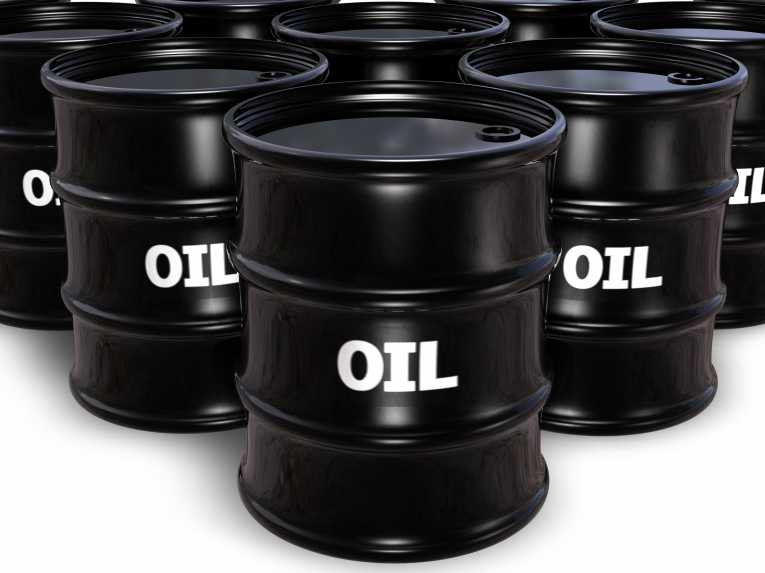
\includegraphics[scale=0.10]{./Chapter1/Figures/figure-oil.jpg}};
\node [anchor=north west] (part1text) at ([xshift=-1em,yshift=0.0em]part1label.south west) {\begin{tabular}{l}{\color{red}{资源}}:可以使机器翻译\\系统运行的“汽油”\end{tabular}};
\end{scope}
}

{
\begin{scope}[yshift=-1.0in,xshift=2.8in]
\node [] (part2label) at (0,0) {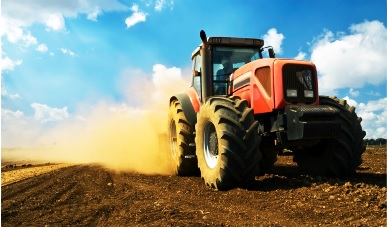
\includegraphics[scale=0.33]{./Chapter1/Figures/figure-truck.jpg}};
\node [anchor=north west] (part2text) at ([xshift=-1em,yshift=0em]part2label.south west) {\begin{tabular}{l}{\color{red}{系统}}:利用资源完成\\自动翻译的程序\end{tabular}};
\end{scope}
}

{
\draw[<-,thick] (part1label.north)..controls +(north:0.6) and +(south:0.6)..([yshift=0.2em]part1.south);
}

{
\draw[<-,thick] ([yshift=0.0em]part2label.north)..controls +(north:0.6) and +(south:0.6)..([yshift=0.2em]part2.south);
}

\end{tikzpicture}


